\documentclass[10pt,preprint]{../aastex}

\usepackage{amsfonts}
\usepackage{amsmath}
\usepackage{amssymb}
\usepackage{amsthm}
\usepackage{booktabs}
\usepackage{mathrsfs}
\usepackage{cite}
\usepackage{times}
\usepackage{url}
\usepackage{hyperref}
\usepackage{lineno}
\usepackage{yhmath}
\usepackage{natbib}
\usepackage{../../definitions}
\hypersetup{
  bookmarksnumbered = true,
  bookmarksopen=false,
  pdfborder=0 0 0,         % make all links invisible, so the pdf looks good when printed
  pdffitwindow=true,      % window fit to page when opened
  pdfnewwindow=true, % links in new window
  colorlinks=true,           % false: boxed links; true: colored links
  linkcolor=blue,            % color of internal links
  citecolor=magenta,    % color of links to bibliography
  filecolor=magenta,     % color of file links
  urlcolor=cyan              % color of external links
}

\usepackage{float}
\usepackage{graphicx}
\newtheorem{remark}{Remark}
\graphicspath{{Figures/}}
\newcommand{\figref}[1]{Figure \ref{#1}}

\begin{document}
Throughout this document, lowercase latin indices ($i,j,$ etc.) run from 1 to 3, lowercase Greek indices ($\mu,\nu,$ etc.) run from 0 to 3, and uppercase latin indices ($J$) run from 1 to 5.

\section{Equations}
We are solving the general relativistic hydrodynamics (GRH) equations \citep{RezzollaRelHyd}:
\begin{equation}\label{Eq:GRH}
\pd{\left(\sqrt{\gamma}\,\bU\right)}{t}+\pd{\left(\alpha\,\sqrt{\gamma}\,\bF^{i}\right)}{i}=\sqrt{\gamma}\,\bS,
\end{equation}
where $\bU$ is the vector of conserved variables, defined as
\begin{equation}
\bU\longrightarrow U^{J}=\begin{pmatrix}D\\ S_{j}\\ E\end{pmatrix}=\begin{pmatrix}\rho\,W\\ \rho\,h\,W^{2}\,v_{j}\\\rho\,h\,W^{2}-p\end{pmatrix},
\end{equation}
$\bF^{i}$ is the vector of fluxes of the conserved variables in the $x^{i}$-direction, defined as
\begin{equation}
\bF^{i}\longrightarrow \left(F^{i}\right)^{J}=\begin{pmatrix}D\left(v^{i}-\eta^{i}\right)\\ S_{j}\left(v^{i}-\eta^{i}\right)+p\,\delta^{i}_{~j}\\S^{i}-\eta^{i}\,E\end{pmatrix},
\end{equation}
$\bS$ is the vector of sources, defined as
\begin{equation}
\bS\longrightarrow S^{J}=\begin{pmatrix}0\\\frac{1}{2}\,\alpha\,P^{ik}\,\pd{\gamma_{ik}}{j}+S_{i}\,\pd{\beta^{i}}{j}-E\,\pd{\alpha}{j}\\\alpha\,P^{ij}\,K_{ij}-S^{j}\,\pd{\alpha}{j}\end{pmatrix},
\end{equation}
where $\rho$ is the mass-density of the fluid, $v^{i}$ are the contravariant components of the fluid three-velocity, and $p$ is the pressure of the fluid. The quantity $h$ is the specific enthalpy of the fluid, defined as
\begin{equation}
h\equiv1+\frac{e+p}{\rho},
\end{equation}
where $e$ is the internal energy-density of the fluid. The quantity $W$ is the Lorentz factor of the fluid, defined as
\begin{equation}
W\equiv\left(1-\vv{v}\cdot\vv{v}\right)^{-1/2}.
\end{equation}
The quantity $\alpha$ is the lapse function, $\eta^{i}$ are the ratio of the components shift-vector, $\beta^{i}$, to the lapse function:
\begin{equation}
\vv{\eta}\longrightarrow\eta^{i}\equiv\alpha^{-1}\,\beta^{i},
\end{equation}
and $\gamma_{ij}$ are the covariant components of the spatial three-metric tensor, i.e. $\gamma^{ij}\,\gamma_{jk}=\delta^{i}_{~k}$, where $\delta^{i}_{~k}$ are the usual components of the Kronecker delta tensor. The $P^{ij}$ are the components of the stress-tensor, defined as
\begin{equation}
\bP\longrightarrow P^{ij}\equiv\rho\,h\,W^{2}\,v^{i}\,v^{j}+p\,\gamma^{ij},
\end{equation}
and the $K_{ij}$ are the components of the extrinsic curvature, defined as
\begin{equation}
\text{FILL IN HERE}.
\end{equation}

\section{Derivation of Middle Wave-Speed Estimate for General Relativistic HLLC Numerical Flux}
For a given Riemann problem we assume that a discontinuity breaks up into four distinct regions (see \figref{Fig:HLLC_RiemannFan}).
\begin{figure}[H]
\centering
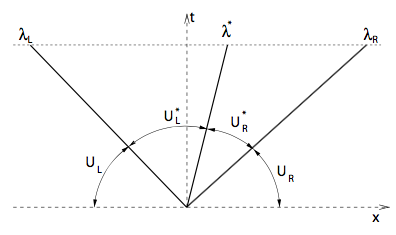
\includegraphics[scale=0.5]{HLLC_RiemannFan_MB2005}
\caption{HLLC Riemann fan from \citet{Mignone2005}.}\label{Fig:HLLC_RiemannFan}
\end{figure}

\subsection{Derivation of Rankine-Hugoniot Jump Conditions}
This derivation closely follows \citet{RezzollaRelHyd}.

We start the derivation by integrating the one-dimensional version of \eqref{Eq:GRH} in space from a point $x_{L}$ to a point $x_{R}$, that contains a shock, which we define to be at a time-dependent point $x_{L}<\lambda\left(t\right)<x_{R}$:
\begin{equation}
\int\limits_{x_{L}}^{x_{R}}\pd{\left(\sqrt{\gamma}\,\bU\right)}{t}\,dx+\int\limits_{x_{L}}^{x_{R}}\pd{\left(\alpha\,\sqrt{\gamma}\,\bF^{x}\right)}{x}\,dx=\int\limits_{x_{L}}^{x_{R}}\sqrt{\gamma}\,\bS\,dx.
\end{equation}
First, we note that in the first integral on the LHS we can pull out the partial derivative with respect to time, which converts it into a total derivative. We also perform an integration-by-parts on the second integral on the LHS, yielding
\begin{align}
\frac{d}{dt}\int\limits_{x_{L}}^{x_{R}}&\sqrt{\gamma}\,\bU\,dx+\left[\alpha\,\sqrt{\gamma}\,\bF^{x}\right]^{x_{R}}_{x_{L}}=\int\limits_{x_{L}}^{x_{R}}\sqrt{\gamma}\,\bS\,dx\\
&\implies\frac{d}{dt}\int\limits_{x_{L}}^{x_{R}}\sqrt{\gamma}\,\bU\,dx+\alpha_{R}\,\sqrt{\gamma_{R}}\,\bF_{R}^{x}-\alpha_{L}\,\sqrt{\gamma_{L}}\,\bF_{L}^{x}=\int\limits_{x_{L}}^{x_{R}}\sqrt{\gamma}\,\bS\,dx,
\end{align}
where $\alpha_{L}=\alpha\left(x_{L}\right)$, etc. The integral over the vector of conserved variables contains the discontinuity, and therefore it's derivative is not well-defined. To overcome this we split the integral into one integral from $x_{L}$ to the location of the shock as approached from below, $s^{-}\left(t\right)$, and another integral from the location of the shock as approached from above, $s^{+}\left(t\right)$, to $x_{R}$:
\begin{equation}
\int\limits_{x_{L}}^{x_{R}}\sqrt{\gamma}\,\bU\,dx=\int\limits_{x_{L}}^{s^{-}\left(t\right)}\sqrt{\gamma}\,\bU\,dx+\int\limits_{s^{+}\left(t\right)}^{x_{R}}\sqrt{\gamma}\,\bU\,dx.
\end{equation}
Both of these integrals are smooth. Next we use the rule for differentiation of an integral depending on a parameter \citep{RezzollaRelHyd}:
\begin{equation}
\f{d}{dt}\int\limits_{x_{1}\left(t\right)}^{x_{2}\left(t\right)}Q\left(x,t\right)\,dx=\int\limits_{x_{1}\left(t\right)}^{x_{2}\left(t\right)}\pd{Q\left(x,t\right)}{t}\,dx+Q\left(x_{2}\left(t\right),t\right)\,\frac{dx_{2}\left(t\right)}{dt}-Q\left(x_{1}\left(t\right),t\right)\,\frac{dx_{1}\left(t\right)}{dt}.
\end{equation}
This yields, since $x_{L}$ and $x_{R}$ are constant,
\begin{align}
\int\limits_{x_{L}}^{s^{-}\left(t\right)}&\pd{\left(\sqrt{\gamma}\,\bU\right)}{t}\,dx+\sqrt{\gamma\left(s^{-}\left(t\right),t\right)}\,\bU\left(s^{-}\left(t\right),t\right)\,\frac{ds^{-}}{dt}\\
&+\int\limits_{s^{+}\left(t\right)}^{x_{R}}\pd{\left(\sqrt{\gamma}\,\bU\right)}{t}\,dx-\sqrt{\gamma\left(s^{+}\left(t\right),t\right)}\,\bU\left(s^{+}\left(t\right),t\right)\,\frac{ds^{+}}{dt}\\
&+\alpha_{R}\,\sqrt{\gamma_{R}}\,\bF_{R}-\alpha_{L}\,\sqrt{\gamma_{L}}\,\bF_{L}=\int\limits_{x_{L}}^{x_{R}}\sqrt{\gamma}\,\bS\,dx.
\end{align}
We will now take the limit that $x_{L}\longrightarrow s^{-}$ and $x_{R}\longrightarrow s^{+}$. When we do this, we see that the integrals vanish, because the integrands are all smooth in the regions considered. This yields (defining $\bU_{L}\equiv\bU\left(s^{-}\left(t\right),t\right)$, etc.)
\begin{equation}
\sqrt{\gamma_{L}}\,\bU_{L}\,\frac{ds_{L}}{dt}-\sqrt{\gamma_{R}}\,\bU_{R}\,\frac{ds_{R}}{dt}=\alpha_{L}\,\sqrt{\gamma_{L}}\,\bF_{L}-\alpha_{R}\,\sqrt{\gamma_{R}}\,\bF_{R}.
\end{equation}
Now, we note that $s_{L}=s_{R}$, and that geometry fields are continuous across discontinuities, which means that the metric determinant cancels. This yields, defining the middle wave-speed $\lambda$ as
\begin{equation}
\lambda\equiv\frac{ds}{dt},
\end{equation}
\begin{equation}
\lambda\left(\bU_{L}-\bU_{R}\right)=\alpha\left(\bF_{L}-\bF_{R}\right).
\end{equation}
These are the \textit{Rankine-Hugoniot jump conditions} and they describe how the fluid variables change across a discontinuity. Next we derive an expression for an estimate of the value of the middle wave-speed, $\lambda$.

\subsection{Derivation of Estimate of Middle Wave-Speed $\lambda$}
Now we apply the jump conditions to the shocked and un-shocked fluid (either the left or the right state):
\begin{equation}
\lambda^{i}\left(\bU^{*}-\bU\right)=\alpha\left(\left(\bF^{*}\right)^{i}-\bF^{i}\right).
\end{equation}
We will use the shorthand notation:
\begin{equation}
\bF^{*i}=\left(\bF^{*}\right)^{i}.
\end{equation}
Recalling that the geometry fields are continuous, we assume that the flux in the shocked region can be written as
\begin{equation}
\bF^{*i}\longrightarrow\left(F^{*i}\right)^{J}=\begin{pmatrix}D^{*}\left(\lambda^{*i}-\eta^{i}\right)\\ S^{*}_{j}\left(\lambda^{*i}-\eta^{i}\right)+p^{*}\,\delta^{i}_{~j}\\S^{*i}-\eta^{i}\,E^{*}\end{pmatrix}.
\end{equation}
Applying the jump conditions to the momentum-density equation we get
\begin{align}
\lambda^{i}\left(S_{j}^{*}-S_{j}\right)&=\alpha\left[S^{*}_{j}\left(\lambda^{*i}-\eta^{i}\right)+p^{*}\,\delta^{i}_{~j}-S_{j}\left(v^{i}-\eta^{i}\right)-p\,\delta^{i}_{~j}\right]\\
\implies S^{*}_{j}\left[\lambda^{i}-\alpha\left(\lambda^{*i}-\eta^{i}\right)\right]&=S_{j}\left[\lambda^{i}-\alpha\left(v^{i}-\eta^{i}\right)\right]+\alpha\left(p^{*}-p\right)\delta^{i}_{~j}.
\end{align}
Now we apply the jump conditions to the energy-density equation, which gives
\begin{equation}
\lambda^{i}\left(E^{*}-E\right)=\alpha\left[S^{*i}-\eta^{i}\,E^{*}-S^{i}+\eta^{i}\,E\right].
\end{equation}
Now, we note that
\begin{align}
S^{i}&=\left(E+p\right)v^{i}\label{Eq:Mom-En}\\
S^{*i}&=\left(E^{*}+p^{*}\right)\lambda^{*i}.
\end{align}
Substituting this into the energy-density equation gives
\begin{align}
\lambda^{i}\left(E^{*}-E\right)&=\alpha\left[\left(E^{*}+p^{*}\right)\lambda^{*i}-\eta^{i}\,E^{*}-\left(E+p\right)v^{i}+\eta^{i}\,E\right]\\
\implies E^{*}\left[\lambda^{i}-\alpha\left(\lambda^{*i}-\eta^{i}\right)\right]&=E\left[\lambda^{i}-\alpha\left(v^{i}-\eta^{i}\right)\right]+\alpha\left(p^{*}\,\lambda^{*i}-p\,v^{i}\right).\label{Eq:En1}
\end{align}
Now we substitute \eqref{Eq:Mom-En} into the momentum-density equation which yields
\begin{align}
\left(E^{*}+p^{*}\right)\lambda^{*}_{j}\left[\lambda^{i}-\alpha\left(\lambda^{*i}-\eta^{i}\right)\right]&=S_{j}\left[\lambda^{i}-\alpha\left(v^{i}-\eta^{i}\right)\right]+\alpha\left(p^{*}-p\right)\delta^{i}_{~j}\\
\implies E^{*}\left[\lambda^{i}-\alpha\left(\lambda^{*i}-\eta^{i}\right)\right]\lambda^{*}_{j}&=-p^{*}\left[\lambda^{i}-\alpha\left(\lambda^{*i}-\eta^{i}\right)\right]\lambda^{*}_{j}+S_{j}\left[\lambda^{i}-\alpha\left(v^{i}-\eta^{i}\right)\right]+\alpha\left(p^{*}-p\right)\delta^{i}_{~j}.
\end{align}
Equating this with \eqref{Eq:En1} gives
\begin{align}
&\left\{E\left[\lambda^{i}-\alpha\left(v^{i}-\eta^{i}\right)\right]+\alpha\left(p^{*}\,\lambda^{*i}-p\,v^{i}\right)\right\}\lambda^{*}_{j}\\
&\hspace{5em}=-p^{*}\left[\lambda^{i}-\alpha\left(\lambda^{*i}-\eta^{i}\right)\right]\lambda^{*}_{j}+S_{j}\left[\lambda^{i}-\alpha\left(v^{i}-\eta^{i}\right)\right]+\alpha\left(p^{*}-p\right)\delta^{i}_{~j}.
\end{align}
We see that the term $\alpha\,p^{*}\,\lambda^{*i}\,\lambda^{*}_{j}$ cancels from both sides. We now isolate $p^{*}$ to get
\begin{align}
p^{*}&=\frac{E\left[\lambda^{i}-\alpha\left(v^{i}-\eta^{i}\right)\right]\lambda^{*}_{j}-\alpha\,p\,v^{i}\,\lambda^{*}_{j}-S_{j}\left[\lambda^{i}-\alpha\left(v^{i}-\eta^{i}\right)\right]+\alpha\,p\,\delta^{i}_{~j}}{\alpha\,\delta^{i}_{~j}-\left(\lambda^{i}+\alpha\,\eta^{i}\right)\lambda^{*}_{j}}\\
&=\frac{\left\{E\left[\lambda^{i}-\alpha\left(v^{i}-\eta^{i}\right)\right]-\alpha\,p\,v^{i}\right\}\lambda^{*}_{j}-\left\{S_{j}\left[\lambda^{i}-\alpha\left(v^{i}-\eta^{i}\right)\right]-\alpha\,p\,\delta^{i}_{~j}\right\}}{\alpha\,\delta^{i}_{~j}-\left(\lambda^{i}+\alpha\,\eta^{i}\right)\lambda^{*}_{j}}.
\end{align}
Now we note that
\begin{equation}
E\left[\lambda^{i}-\alpha\left(v^{i}-\eta^{i}\right)\right]-\alpha\,p\,v^{i}=\lambda^{i}\,E-\alpha\left[\left(E+p\right)v^{i}-\eta^{i}\,E\right]=\lambda^{i}\,E-\alpha\left(S^{i}-\eta^{i}\,E\right)=\lambda^{i}\,E-\alpha\,F^{i}_{E},
\end{equation}
and
\begin{equation}
S_{j}\left[\lambda^{i}-\alpha\left(v^{i}-\eta^{i}\right)\right]-\alpha\,p\,\delta^{i}_{~j}=\lambda^{i}\,S_{j}-\alpha\left[S_{j}\left(v^{i}-\eta^{i}\right)+p\,\delta^{i}_{~j}\right]=\lambda^{i}\,S_{j}-\alpha\,F^{i}_{S_{j}}.
\end{equation}
With this, we have
\begin{equation}
p^{*}=\frac{\left(\lambda^{i}\,E-\alpha\,F^{i}_{E}\right)\lambda^{*}_{j}-\left(\lambda^{i}\,S_{j}-\alpha\,F^{i}_{S_{j}}\right)}{\alpha\,\delta^{i}_{~j}-\left(\lambda^{i}+\alpha\,\eta^{i}\right)\lambda^{*}_{j}}.
\end{equation}
Now, since the pressure is continuous across contact discontinuities we can equate the left and right states, giving
\begin{equation}
\frac{\left(-\lambda^{i}_{L}\,E_{L}-\alpha\,F^{i}_{E,L}\right)\lambda^{*}_{j}-\left(-\lambda^{i}_{L}\,S_{j,L}-\alpha\,F^{i}_{S_{j},L}\right)}{\alpha\,\delta^{i}_{~j}-\left(-\lambda^{i}_{L}+\alpha\,\eta^{i}\right)\lambda^{*}_{j}}=\frac{\left(\lambda^{i}_{R}\,E_{R}-\alpha\,F^{i}_{E,R}\right)\lambda^{*}_{j}-\left(\lambda^{i}_{R}\,S_{j,R}-\alpha\,F^{i}_{S_{j},R}\right)}{\alpha\,\delta^{i}_{~j}-\left(\lambda^{i}_{R}+\alpha\,\eta^{i}\right)\lambda^{*}_{j}}.
\end{equation}
Now, cross-multiplying and focusing on the LHS:
\begin{align}
&\left[\alpha\,\delta^{i}_{~j}-\left(\lambda^{i}_{R}+\alpha\,\eta^{i}\right)\lambda^{*}_{j}\right]\left[\left(-\lambda^{i}_{L}\,E_{L}-\alpha\,F^{i}_{E,L}\right)\lambda^{*}_{j}-\left(-\lambda^{i}_{L}\,S_{j,L}-\alpha\,F^{i}_{S_{j},L}\right)\right]\\
&=\left[\alpha\,\delta^{i}_{~j}-\left(\lambda^{i}_{R}+\beta^{i}\right)\lambda^{*}_{j}\right]\left[\left(-\lambda^{i}_{L}\,E_{L}-\alpha\,F^{i}_{E,L}\right)\lambda^{*}_{j}-\left(-\lambda^{i}_{L}\,S_{j,L}-\alpha\,F^{i}_{S_{j},L}\right)\right]\\
&=\alpha\,\delta^{i}_{~j}\left(-\lambda^{i}_{L}\,E_{L}-\alpha\,F^{i}_{E,L}\right)\lambda^{*}_{j}-\alpha\,\delta^{i}_{~j}\left(-\lambda^{i}_{L}\,S_{j,L}-\alpha\,F^{i}_{S_{j},L}\right)\\
&\hspace{3em}-\left(\lambda^{i}_{R}+\beta^{i}\right)\left(-\lambda^{i}_{L}\,E_{L}-\alpha\,F^{i}_{E,L}\right)\left(\lambda^{*}_{j}\right)^{2}+\left(\lambda^{i}_{R}+\beta^{i}\right)\left(-\lambda^{i}_{L}\,S_{j,L}-\alpha\,F^{i}_{S_{j},L}\right)\lambda^{*}_{j}\\
&=-\left(\lambda^{i}_{R}+\beta^{i}\right)\left(-\lambda^{i}_{L}\,E_{L}-\alpha\,F^{i}_{E,L}\right)\left(\lambda^{*}_{j}\right)^{2}\\
&\hspace{3em}+\left[\alpha\,\delta^{i}_{~j}\left(-\lambda^{i}_{L}\,E_{L}-\alpha\,F^{i}_{E,L}\right)+\left(\lambda^{i}_{R}+\beta^{i}\right)\left(-\lambda^{i}_{L}\,S_{j,L}-\alpha\,F^{i}_{S_{j},L}\right)\right]\lambda^{*}_{j}\\
&\hspace{3em}-\alpha\,\delta^{i}_{~j}\left(-\lambda^{i}_{L}\,S_{j,L}-\alpha\,F^{i}_{S_{j,L}}\right).
\end{align}
Expanding out the terms gives
\begin{align}
&\left[\lambda^{i}_{R}\,\lambda^{i}_{L}\,E_{L}+\lambda^{i}_{R}\,\alpha\,F^{i}_{E,L}-\beta^{i}\left(-\lambda^{i}_{L}\,E_{L}-\alpha\,F^{i}_{E,L}\right)\right]\left(\lambda^{*}_{j}\right)^{2}\\
&+\left[\alpha\,\delta^{i}_{~j}\left(-\lambda^{i}_{L}\,E_{L}-\alpha\,F^{i}_{E,L}\right)-\lambda^{i}_{R}\,\lambda^{i}_{L}\,S_{j,L}-\lambda^{i}_{R}\,\alpha\,F^{i}_{S_{j},L}+\beta^{i}\left(-\lambda^{i}_{L}\,S_{j,L}-\alpha\,F^{i}_{S_{j},L}\right)\right]\lambda^{*}_{j}\\
&-\alpha\,\delta^{i}_{~j}\left(-\lambda^{i}_{L}\,S_{j,L}-\alpha\,F^{i}_{S_{j},L}\right).
\end{align}
From symmetry, by letting $L\leftrightarrow R$ and $\lambda^{i}_{L}\leftrightarrow-\lambda^{i}_{R}$, we can immediately write down the RHS as
\begin{align}
&\left[\lambda^{i}_{R}\,\lambda^{i}_{L}\,E_{R}-\lambda^{i}_{L}\,\alpha\,F^{i}_{E,R}-\beta^{i}\left(\lambda^{i}_{R}\,E_{R}-\alpha\,F^{i}_{E,R}\right)\right]\left(\lambda^{*}_{j}\right)^{2}\\
&+\left[\alpha\,\delta^{i}_{~j}\left(\lambda^{i}_{R}\,E_{R}-\alpha\,F^{i}_{E,R}\right)-\lambda^{i}_{R}\,\lambda^{i}_{L}\,S_{j,R}+\lambda^{i}_{L}\,\alpha\,F^{i}_{S_{j},R}+\beta^{i}\left(\lambda^{i}_{R}\,S_{j,R}-\alpha\,F^{i}_{S_{j},R}\right)\right]\lambda^{*}_{j}\\
&-\alpha\,\delta^{i}_{~j}\left(\lambda^{i}_{R}\,S_{j,R}-\alpha\,F^{i}_{S_{j},R}\right).
\end{align}
Now we subtract the LHS from the RHS, giving
\begin{align}
&\left[\lambda^{i}_{R}\,\lambda^{i}_{L}\left(E_{R}-E_{L}\right)-\left(\lambda^{i}_{R}\,\alpha\,F^{i}_{E,L}+\lambda^{i}_{L}\,\alpha\,F^{i}_{E,R}\right)-\beta^{i}\left(\lambda^{i}_{R}\,E_{R}+\lambda^{i}_{L}\,E_{L}+\alpha\,F^{i}_{E,L}-\alpha\,F^{i}_{E,R}\right)\right]\left(\lambda^{*}_{j}\right)^{2}\\
&+\left[\alpha\,\delta^{i}_{~j}\left(\lambda^{i}_{R}\,E_{R}+\lambda^{i}_{L}\,E_{L}+\alpha\,F^{i}_{E,L}-\alpha\,F^{i}_{E,R}\right)-\lambda^{i}_{R}\,\lambda^{i}_{L}\left(S_{j,R}-S_{j,L}\right)+\lambda^{i}_{R}\,\alpha\,F^{i}_{S_{j},L}+\lambda^{i}_{L}\,\alpha\,F^{i}_{S_{j},R}\right.\\
&\hspace{3em}\left.+\beta^{i}\left(\lambda^{i}_{R}\,S_{j,R}+\lambda^{i}_{L}\,S_{j,L}+\alpha\,F^{i}_{S_{j},L}-\alpha\,F^{i}_{S_{j},R}\right)\right]\\
&-\alpha\,\delta^{i}_{~j}\left(\lambda^{i}_{R}\,S_{j,R}+\lambda^{i}_{L}\,S_{j,L}+\alpha\,F^{i}_{S_{j},L}-\alpha\,F^{i}_{S_{j},R}\right).
\end{align}
By making use of the HLL conserved variables and fluxes,
\begin{align}
\left(\lambda^{i}_{R}+\lambda^{i}_{L}\right)\bU_{HLL}&=\lambda^{i}_{R}\,\bU_{R}+\lambda^{i}_{L}\,\bU_{L}+\alpha\,\bF^{i}_{L}-\alpha\,\bF^{i}_{R}\\
\left(\lambda^{i}_{R}+\lambda^{i}_{L}\right)\bF^{i}_{HLL}&=\lambda^{i}_{R}\,\alpha\,\bF^{i}_{L}+\lambda^{i}_{L}\,\alpha\,\bF_{R}-\lambda^{i}_{R}\,\lambda^{i}_{L}\left(\bU_{R}-\bU_{L}\right),
\end{align}
we can simplify the quadratic equation to (assuming that $\lambda^{i}_{L}\neq0$ \textbf{and} $\lambda^{i}_{R}\neq0$)
\begin{equation}
\left(-F^{i}_{E,HLL}-\beta^{i}\,E_{HLL}\right)\left(\lambda^{*}_{j}\right)^{2}+\left[\alpha\,\delta^{i}_{~j}\,E_{HLL}+F^{i}_{S_{j},HLL}+\beta^{i}\,S_{j,HLL}\right]\lambda^{*}_{j}-\alpha\,\delta^{i}_{~j}\,S_{j,HLL}=0.
\end{equation}
Now we just multiply the equation by $-1$, which gives
\begin{equation}
\left(F^{i}_{E,HLL}+\beta^{i}\,E_{HLL}\right)\left(\lambda^{*}_{j}\right)^{2}-\left[\alpha\,\delta^{i}_{~j}\,E_{HLL}+F^{i}_{S_{j},HLL}+\beta^{i}\,S_{j,HLL}\right]\lambda^{*}_{j}+\alpha\,\delta^{i}_{~j}\,S_{j,HLL}=0.
\end{equation}
Finally, we use the metric to raise the index on the contact wave-speed, which gives
\begin{equation}
\left(\gamma_{jk}\right)^{2}\left(F^{i}_{E,HLL}+\beta^{i}\,E_{HLL}\right)\left(\lambda^{*k}\right)^{2}-\gamma_{jk}\left[\alpha\,\delta^{i}_{~j}\,E_{HLL}+F^{i}_{S_{j},HLL}+\beta^{i}\,S_{j,HLL}\right]\lambda^{*k}+\alpha\,\delta^{i}_{~j}\,S_{j,HLL}=0.
\end{equation}

We see that in the special relativistic, Cartesian coordinate limit of $\alpha\rightarrow1$, $\beta^{i}\rightarrow0^{i}$, and $\gamma_{ij}=\delta_{ij}$, we recover the result of \citet{Mignone2005}.

\newpage
\bibliographystyle{../apj}
\bibliography{../../References/references.bib}
\end{document}
